\section{Implementation and Evaluation Protocol}
\label{sec:implementation}

This section separates the protocol that produced the paper's reported results
from settings chosen to make the released reconstruction executable.  It also
defines the unit of inference and the failure-recovery population; without
these distinctions, additional samples, evaluator-guided reranking, or a
different 658-scene checkpoint pair could silently change the claim being
tested.

\subsection{Architecture and Trajectory Interface}
\label{sec:architecture}

AMPT uses the paper-reported InternVL3-2B visual-language backbone and the
ReCogDrive conditional diffusion planner.  The paper describes multi-view
camera features, ego state and motion history, and a discrete high-level
command.  One audited APR command instead resolves \texttt{cam\_type=single};
because the exact final checkpoint manifest is incomplete, this is recorded as
a protocol discrepancy rather than silently attributed to every reported row.
The planning head predicts a four-second ego trajectory as eight
poses at 0.5-second spacing, stored as an $8\times3$ tensor of local-frame
$(x,y,\mathrm{heading})$.  The VLM context conditions every diffusion step;
the supervised objective samples a noisy version of one target trajectory and
regresses the corresponding diffusion noise.

The archived agent configuration sets \texttt{train\_backbone=false} and the
planner accepts cached VLM features.  Accordingly, the \emph{proposed
reproduction} freezes InternVL3-2B and optimizes the ReCogDrive diffusion
planner in all four training phases.  This makes the supervision variants
differ only in target construction and makes the policy-optimization variants
differ only in credit and refinement.  The archived planner default uses five
DDIM denoising steps; the proposed rerun keeps five steps for rollout sampling,
log-probability evaluation, and final inference.  A random training diffusion
timestep is still used for ordinary denoising supervision.

\subsection{Stage-Wise Training Protocol}
\label{sec:training-protocol}

The main paper reports 200 epochs for GT-only and multi-trajectory imitation
learning, 16 rollouts per scene and 10 epochs for GRPO, three APR rounds, and
eight NVIDIA A800 GPUs.  An archived historical Core-Pareto launcher contains
20 epochs; because it is not the resolved manifest for the reported run, it is
not used to overwrite the paper's 10-epoch protocol.  One audited APR branch
used AdamW, BF16, four GPUs, per-GPU batch size eight (global batch 32), learning
rate $5\times10^{-7}$ with minimum $2.5\times10^{-7}$, three epochs, advantage
temperature 0.05, and weight clip 5.  We identify those values as
\emph{branch-verified}, not as proof that every reported APR round used an
identical schedule.

The table marks each row as reported, branch-verified, historical, or
\emph{proposed reproduction}.  Where the final manifest is unresolved, the
proposed schedule uses AdamW with $(\beta_1,\beta_2)=(0.9,0.95)$, weight decay
$10^{-4}$, BF16, norm clipping at 1.0, and cosine decay.  GT-only and PC-MTS use
learning rate $10^{-4}$, a three-epoch warmup, minimum learning rate $10^{-6}$,
eight scenes per GPU and two-step gradient accumulation on eight GPUs (global
batch 128).  FF-PGRPO uses $10^{-4}$, two groups per GPU, four-step
accumulation on eight GPUs (64 scene groups per update), the paper's 16
rollouts per group, and the regularization schedule in
Section~\ref{sec:ff-pgrpo-details}.  APR follows the branch-verified optimizer
settings and trains three epochs per promoted round.  Proposed training seeds
are 20260726, 20260727, and 20260728; they are future rerun identifiers and are not assigned
to any existing point estimate.

\begin{table*}[t]
\centering
\small
\caption{Stage-wise training protocol. Reported/reproduced settings are distinguished from bounded reproduction settings; `not recorded' is an explicit provenance value, not a blank. Inference always emits one trajectory.}
\label{tab:stage_hyperparameters}
\resizebox{\textwidth}{!}{%
\begin{tabular}{lccccc}
\toprule
field & GT-only & PC-MTS & FF-PGRPO & APR & status \\
\midrule
Target & logged GT & one sampled GT/candidate & sampled policy trajectories & audited teacher + policy retention & mixed provenance \\
Epochs & 200 & 200 & 10 & 3 per audited branch; 3 paper rounds & paper reported / APR branch reproduced \\
Optimizer & AdamW & AdamW & AdamW & AdamW & historical implementation / reproduction setting \\
Peak learning rate & 1e-4 & 1e-4 & 1e-4 & 5e-7 & historical configs / APR reproduced \\
Minimum learning rate & 1e-6 & 1e-6 & 1e-6 & 2.5e-7 & historical configs / APR reproduced \\
Weight decay & 1e-4 & 1e-4 & 1e-4 & 1e-4 & historical / proposed for APR \\
Batch per GPU & 8 & 8 & 2 & 8 & historical / FF and APR manifests \\
GPUs & 8 & 8 & 8 & 4 & paper reports 8 overall; APR branch used 4 \\
Gradient accumulation & 2 & 2 & 4 & 1 & historical / FF and APR manifests \\
Effective batch & 128 & 128 & 64 & 32 & deterministic from rows above \\
Precision & bf16-mixed & bf16-mixed & bf16-mixed & bf16-mixed & historical / APR reproduced \\
Warmup epochs & 3 & 3 & not recorded & 0 & historical / APR reproduced \\
Gradient clipping & 1.0 & 1.0 & 1.0 & 1.0 & historical / proposed where unresolved \\
Rollouts per scene & not applicable & 16 support rollouts & 16 & 8 offline candidates & proposed PC-MTS; paper FF; APR manifest \\
Advantage temperature & not applicable & not applicable & group normalized & 0.05 & APR reproduced \\
Advantage/weight clip & not applicable & not applicable & 3.0 & 5.0 & historical FF default / APR reproduced \\
BC or retention weight & not applicable & not applicable & 0.10 to 0.05 & 1.0 retention & archived FF / APR reproduced \\
Reference KL & not applicable & not applicable & 0.02 & 0.02 prior distance & archived FF / APR reproduced \\
Inference trajectories & 1 & 1 & 1 & 1 & paper and submission provenance \\
\bottomrule
\end{tabular}%
}
\end{table*}


No new multi-GPU training was started for this supplement.  The launchers are
dry-run by default and require both \texttt{ALLOW\_TRAIN=1} and an explicit
\texttt{--execute} flag.  Wall-clock time and
storage are explicitly recorded as \emph{not measured}; no scheduler estimate
is presented as an experiment.  Offline cost is reported in evaluator calls
rather than guessed wall
time: one call per retained scene trajectory for a benchmark evaluation, eight
additional calls per Stage-1 robustness center under the proposed tube, and at
most four calls per APR teacher under the proposed interpolation list.  Every
future launch records wall time, peak device memory, output bytes, resolved
configuration, Git revision, and SHA-256 hashes.

\subsection{Benchmark Evaluation}
\label{sec:evaluation-protocol}

\paragraph{NAVSIM v1.}
The scene-level reproduced export contains 12,146 single-trajectory predictions
on \texttt{navtest}; 12,138 have metric caches and are scored.  Their mean is
PDMS 0.9145046521, with NC 0.9852941176, DAC 0.9798978415, TTC
0.9600428407, comfort 1.0, and EP 0.8674798204.  These reproduce the rounded
91.4/98.5/98.0/96.0/100/86.7 row in the main paper.  The archived inference
seed is 20260726.  The eight unscored predictions are excluded from component
and aggregate means and remain listed in provenance; they are not imputed.
The scorer implementation is mapped to
\path{ba5908d:navsim/evaluate/pdm_score.py:pdm_score}.

\paragraph{NAVSIM v2.}
The reproduced \texttt{navtest} export has 12,146 successful trajectories and
mean EPDMS 0.8911677436.  Its component means reproduce the rounded main-paper
row: NC 98.4, DAC 97.7, DDC 99.0, TLC 99.7, TTC 97.7, EP 89.4, LK 91.7, HC
97.1, and EC 87.7.  The official evaluator revision recorded with this export
is \texttt{0a380a9063d7162ec93d0f51e9990ebac585f720}.  EC has 10,040 direct
per-scene values and is aggregated by the official evaluator; we do not
pretend that the other 2,106 rows contain directly observed EC entries.

\begin{table*}[t]
\centering
\small
\caption{Scene-level reproduction of the AMPT main results under one-trajectory inference without test-time scoring or reranking. All metrics are percentages and higher is better. NAVSIM v1 has 12,138 scored scenes; v2 has 12,146.}
\label{tab:reproduced_main}
\resizebox{\textwidth}{!}{%
\begin{tabular}{lccccccccccccccc}
\toprule
Benchmark & Scenes & Inference & Runs & NC & DAC & TTC & C & EP & PDMS & DDC & TLC & LK & HC & EC & EPDMS \\
\midrule
NAVSIM v1 & 12138 & 1 trajectory & 1 archived inference seed & 98.53 & 97.99 & 96.00 & 100.00 & 86.75 & 91.45 & not recorded & not recorded & not recorded & not recorded & not recorded & not recorded \\
NAVSIM v2 & 12146 & 1 trajectory & 1 export; seed not recorded & 98.42 & 97.69 & 97.66 & not recorded & 89.45 & not recorded & 99.00 & 99.71 & 91.73 & 97.09 & 87.74 & 89.12 \\
\bottomrule
\end{tabular}%
}
\end{table*}


\begin{figure*}[t]
  \centering
  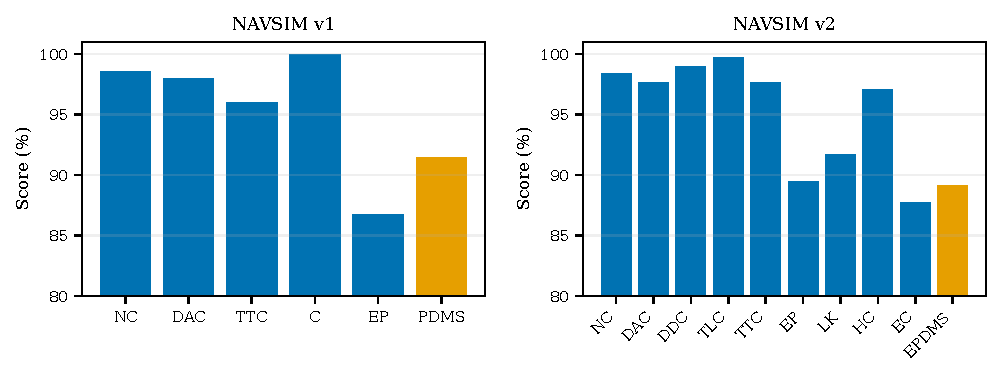
\includegraphics[width=0.76\textwidth]{figures/generated/ampt_metric_profiles.pdf}
  \caption{Scene-level reproduced AMPT component profiles on NAVSIM v1 and
  v2.  All metrics are percentages and higher is better; aggregate PDMS/EPDMS
  is shown in orange.  The profiles use 12,138 and 12,146 scored scenes,
  respectively, from one inference realization.}
  \label{fig:metric-profiles}
\end{figure*}

\paragraph{Single-trajectory inference.}
For each scene and inference seed, the model receives one observation, runs one
five-step denoising chain, and submits its single final $8\times3$ trajectory.
There is no test-time group sampling, evaluator call, candidate scoring,
reference lookup, model ensemble, or reranking.  The v1 submission provenance
independently records candidate count one, so this is a scene-level reproduced
property rather than only a methodological statement.

\paragraph{Runs and uncertainty.}
The archived v1/v2 headline exports each establish a scene-level mean for one
policy realization; they do not establish across-seed variance.  We therefore
do not attach a fabricated standard deviation to the 0.1--0.3 point increments
in the paper.  For the proposed rerun, each of seeds
20260726/20260727/20260728 produces a
complete scene export.  We first compute the mean for each run and report the
mean $\pm$ standard deviation across the three runs.  Method differences use
10,000 paired bootstrap resamples of shared scenes (resampling seeds and then
scenes within seed when multiple seeds are present), with a fixed analysis seed
of 2027 and a two-sided 95\% interval.  Recovery proportions use Wilson 95\%
intervals.  Scene bootstrap intervals from one model run describe variation
over the evaluated scenes and are explicitly not interpreted as training-seed
stability.

\paragraph{Model selection disclosure.}
The archived final v1 provenance states that \texttt{navtest} participated in
checkpoint selection.  We therefore describe the headline table as a
paper-reported benchmark comparison, not as a clean held-out model-selection
study.  The proposed rerun selects checkpoints only on the training/validation
partition, seals a checkpoint hash before \texttt{navtest}, and evaluates each
sealed hash once per inference seed.  This disclosure does not change a main
paper number; it narrows the fairness claim to what the available provenance
supports.

\subsection{The Fixed 658-Scene Recovery Protocol}
\label{sec:hard658-protocol}

The hard population is fixed before comparing optimization methods.  A scene
enters the set when the ReCogDrive IL policy receives PDMS zero in all five
sampling attempts because of collision, drivable-area violation, or both.
The resulting intersection contains 658 scene IDs.  A method \emph{recovers} a
scene when its single submitted trajectory has PDMS strictly greater than
zero under the same evaluator; the threshold is not retuned per method.

For consistency with the main paper, every supplementary hard-set analysis
uses the same archived scalar-GRPO versus historical Core-Pareto recovery pair that produced
367 and 440 positive-score scenes.  It does not substitute a later
full-benchmark checkpoint.  On the 658 fixed scenes, scalar GRPO has 367
positive and 291 zero-score outcomes, whereas the manuscript recovery
checkpoint has 440 positive and 218 zero-score outcomes.  Their paired
transition counts are 347 retained successes, 20 new failures, 93 repaired
failures, and 198 persistent failures.  Hence the net recovery is
$93-20=73$ scenes, exactly the change $440-367$, rather than a gain obtained by
hiding newly failed scenes.  The corresponding recovery rates are 55.8\%
(Wilson 95\% CI 52.0--59.5; $n=658$) and 66.9\% (63.2--70.4; $n=658$).  A
10,000-sample paired scene bootstrap gives an absolute difference of 11.1
percentage points with a 95\% interval of 8.1--14.3 points.
These intervals describe one archived checkpoint pair; no training-seed
identifier was retained for this hard-set export.

The fixed-set construction contains 480 DAC-only, 165 collision-only, and 13
joint collision-and-DAC cases according to the archived cause manifest.  The
same IDs and failure labels are used in all hard-set transition and case-table
analyses.  In particular, ``440 recovered'' means 440 positive outcomes on the
fixed original population; the transition table is required whenever the
claim is interpreted as a policy-to-policy improvement.

\subsection{Baseline and Controlled-Comparison Protocol}
\label{sec:baseline-protocol}

\begin{table*}[t]
\centering
\small
\caption{Fair-comparison protocol for main-paper baselines. All methods use one inference candidate and no test-time scorer in the paper table; unreported backbone/sensor/data details are not inferred. Result identity distinguishes reported from reproduced.}
\label{tab:baseline_protocol}
\resizebox{\textwidth}{!}{%
\begin{tabular}{lcccccc}
\toprule
method & backbone & sensors & training\_data & inference\_candidates & test\_time\_scorer & result\_identity \\
\midrule
AMPT & InternVL3-2B + ReCogDrive diffusion planner & multi-view in paper; one audited APR command resolves single camera & NAVSIM plus offline candidate/teacher pools & 1 & no & locally reproduced v1/v2 final rows; camera-manifest discrepancy disclosed \\
ReCogDrive & not disclosed in current PDF & not disclosed in current PDF & not disclosed in current PDF & 1 & no & paper reported \\
DiffusionDriveV2 & not disclosed in current PDF & not disclosed in current PDF & not disclosed in current PDF & 1 & no & paper reported \\
Drive-JEPA & not disclosed in current PDF & not disclosed in current PDF & not disclosed in current PDF & 1 & no & paper reported \\
\bottomrule
\end{tabular}%
}
\end{table*}


AMPT's v1 and v2 rows are locally reproduced from scene-level outputs.  Other
headline baseline rows are values reported in the main paper and their cited
sources; no local checkpoint, common prediction export, or common seed manifest
was found for them.  They are consequently labeled \emph{reported}, not
\emph{reproduced}.  The table records backbone, sensor interface, training
data, number of inference candidates, and use of a test-time scorer whenever
the cited evidence establishes those fields.  An unavailable field is marked
``not established by the audited source'' rather than filled by analogy with
AMPT.

For the GT/Score/Pareto/PC-MTS comparison, the paper reports a shared
initialization, diffusion SFT loss, optimizer, epoch budget, scalar-GRPO
configuration, and evaluation protocol.  The controlled reproduction
additionally seals the candidate-source manifest, fixes the proposed non-GT
sampling probability, matches the accepted candidate count, draws one target
per scene-update, and uses the same three proposed training seeds.  For Scalar GRPO versus FF-PGRPO, all rollout
chains are generated from the same initialization and sampled with the same
seed before the credit function is changed.  For No APR versus Full APR, total
optimizer steps are matched by continuing the no-APR policy with retention
targets.  These are proposed control procedures until their launch manifests
and outputs exist; the main-paper point estimates remain labeled
paper-reported.

\subsection{Reproduction and Integrity Checks}
\label{sec:reproduction-checks}

The canonical dataset stores normalized scores, benchmark and split, method,
stage, variant, round, scene ID, seed when recorded, feasibility/failure
transitions, teacher status, and its source-file/key provenance.  Validation
checks expected scene counts, duplicate scene-method records, score ranges,
the benchmark aggregate formulas, paired scene sets, and failure-state logic.
Final tables and figures are generated from that dataset; a validation failure
stops manuscript generation.  The build manifest records the command, analysis
seed, package versions, Git revision, and SHA-256 hashes of inputs and outputs.
All raw result directories are read-only, and all derived files remain under
the supplementary directory.
